\subsection{Absolute Maximum Ratings}
\textbf{Caution:} These are stress ratings only. Full operation is not guaranteed while operating outside of the specification defined in \autoref{section:dc-characteristics}.

\begin{table}[h]
    \begin{tabularx}{\textwidth}{
    % Column width scale factors (\hsize=) must all add up to 1
    | >{\hsize=0.1\hsize\centering\arraybackslash}X 
    | >{\hsize=0.45\hsize}X 
    | >{\hsize=0.15\hsize\centering\arraybackslash}X 
    | >{\hsize=0.15\hsize\centering\arraybackslash}X 
    | >{\hsize=0.15\hsize\centering\arraybackslash}X |
    }
        \hline
        \rowcolor{lightgray!50}
        \textbf{Symbol} &
        \textbf{Parameter} &
        \textbf{Min} &
        \textbf{Max} &
        \textbf{Unit} \\
        \hline
        V\textsubscript{DD} & DC Supply Voltage & 4.75 & 5.25 & V \\
        \hline
        V\textsubscript{IO} & GPIO Voltage & -0.3 & 3.5 & V \\
        \hline
        I\textsubscript{IO} & GPIO Current & -8 & 8 & mA \\
        \hline
        V\textsubscript{ADC} & ADC Input Voltage & -0.3 & 3.6 & V \\
        \hline
        I\textsubscript{REG} & Total Output Current of Voltage Regulator & --- & 2 & A \\
        \hline
        T\textsubscript{A} & Operating Temperature & -40 & 85 & °C \\
        \hline
        T\textsubscript{S} & Storage Temperature & -40 & 85 & °C \\
        \hline
    \end{tabularx}
    \caption{Absolute Maximum Ratings}
\end{table}

\subsection{DC Characteristics} \label{section:dc-characteristics}
\begin{table}[h]
    \begin{tabularx}{\textwidth}{
    % Column width scale factors (\hsize=) must all add up to 1
    | >{\hsize=0.1\hsize\centering\arraybackslash}X 
    | >{\hsize=0.4\hsize}X 
    | >{\hsize=0.1\hsize\centering\arraybackslash}X 
    | >{\hsize=0.1\hsize\centering\arraybackslash}X 
    | >{\hsize=0.1\hsize\centering\arraybackslash}X 
    | >{\hsize=0.1\hsize\centering\arraybackslash}X |
    }
        \hline
        \rowcolor{lightgray!50} 
        \textbf{Symbol} &
        \textbf{Parameter} &
        \textbf{Min} &
        \textbf{Typ} &
        \textbf{Max} &
        \textbf{Unit} \\
        \hline
        V\textsubscript{DD} & DC Supply Voltage & 4.75 & 5.00 & 5.25 & V \\
        \hline
        V\textsubscript{IH} & GPIO Input High & 2.0 & 3.3 & 3.5 & V \\
        \hline
        V\textsubscript{IL} & GPIO Input Low & -0.3 & 0 & 0.8 & V \\
        \hline
        V\textsubscript{OH} & GPIO Output High & 2.9 & 3.3 & 3.3 & V \\
        \hline
        V\textsubscript{OL} & GPIO Output Low & 0 & 0 & 0.4 & V \\
        \hline
        V\textsubscript{ADC} & ADC Input Range & 0 & --- & 3.3 & V \\
        \hline
    \end{tabularx}
    \caption{DC Characteristics}
\end{table}

\newpage

\subsection{Power Supply Options}
The ETH4K has three power supply options: the micro USB connector, the screw terminal, and the 5V pins in I/O Bank C. The Texas Instruments TPS2116 Power MUX is used for keeping these sources isolated (see \autoref{figure:power-schematic}).

The power MUX always selects the screw terminal supply over the USB supply unless the screw terminal voltage falls below 4.75V. This allows the device to be programmed and communicate over USB while drawing power from another supply. It also allows the USB cable to safely be connected/disconnected during operation.

The 5V pins in I/O Bank C are connected directly to the 5V net. The power MUX prevents reverse currents from flowing into the screw terminal supply and USB supply, but it cannot prevent reverse currents from flowing into the external supply connected to this 5V net. Always ensure that your supply circuitry has adequate reverse current protection.

Other than removing the USB cable, the power supply option should not be switched during operation. This can cause the supply voltage to momentarily drop, leading to unexpected glitches or even a reset event to occur. Power off the device before changing the power supply option.

% Power Schematic Figure
\begin{figure}[ht]
    \centering
    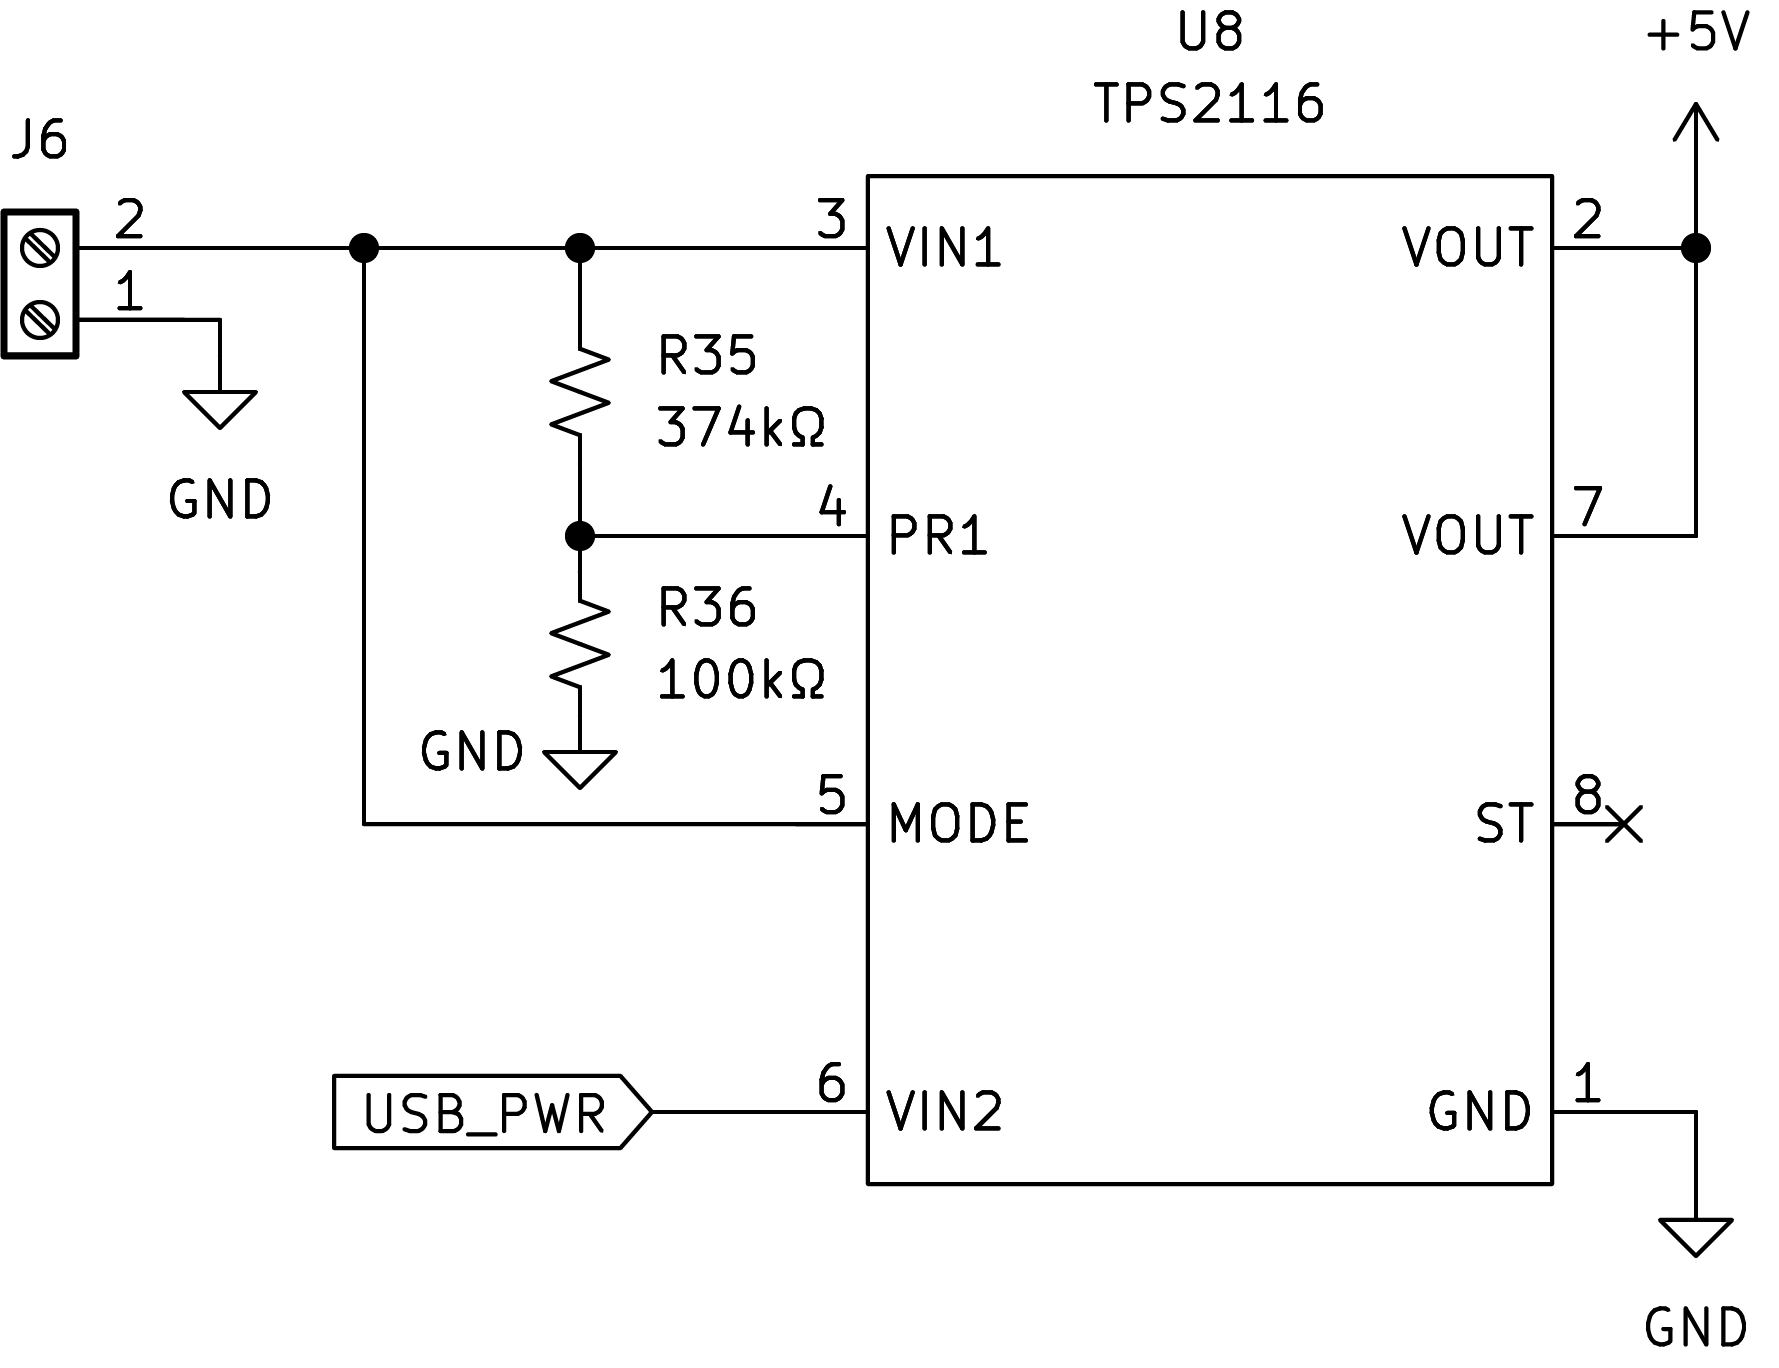
\includegraphics[width=8.25cm]{assets/power-schematic.png}
    \caption{Power MUX Schematic Diagram}
    \label{figure:power-schematic}
\end{figure}

\vspace{12pt}

\textbf{Caution:} Please refrain from touching the ETH4K with bare hands during operation. The power supply circuitry is tuned with precision resistors and is particularly sensitive to the parasitic resistances introduced from bare skin (especially wet hands).

\newpage